% document formatting
\documentclass[10pt]{article}
\usepackage[utf8]{inputenc}
\usepackage[left=1in,right=1in,top=1in,bottom=1in]{geometry}
\usepackage[T1]{fontenc}
\usepackage{xcolor}

% math symbols, etc.
\usepackage{amsmath, amsfonts, amssymb, amsthm}

% lists
\usepackage{enumerate}

% images
\usepackage{graphicx} % for images
\usepackage{tikz}

% code blocks
\usepackage{minted, listings} 

% verbatim greek
\usepackage{alphabeta}

\newcommand{\dd}{\text{d}}
\newcommand{\pr}{\text{Pr}}

\graphicspath{{./assets/images/Week 10}}

\title{02-712 Week 10 \\ \large{Biological Modeling and Simulation}}
 
\author{Aidan Jan}

\date{\today}

\begin{document}
\maketitle

\subsection*{Ergolic Graphs}
An Ergolic graph is one where every state is reachable from every other state with a non-zero probability.  Suppose we have an ergodic graph with states:
\[Q = (q_1, q_2, q_3, q_4, q_5)\]
which includes transitions in both directions between:
$(q_1, q_2), (q_2, q_3), (q_3, q_4), (q_4, q_5), (q_2, q_5)$.  Note that $q_2$ has the highest degree in the graph (degree 3).
\begin{center}
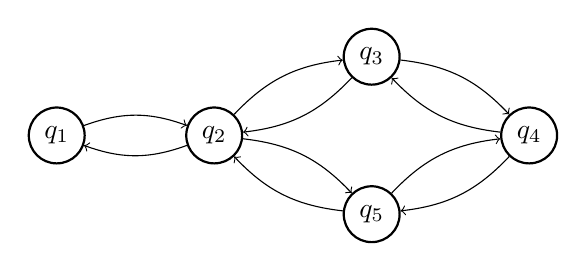
\begin{tikzpicture}
    \node[thick, circle, draw] at (0, 0) (q1) {$q_1$};
    \node[thick, circle, draw] at (2, 0) (q2) {$q_2$};
    \node[thick, circle, draw] at (4, 1) (q3) {$q_3$};
    \node[thick, circle, draw] at (6, 0) (q4) {$q_4$};
    \node[thick, circle, draw] at (4, -1) (q5) {$q_5$};
    
    \draw[->, bend left=20] (q1) to (q2); \draw[->, bend left=20] (q2) to (q1);
    \draw[->, bend left=20] (q2) to (q3); \draw[->, bend left=20] (q3) to (q2);
    \draw[->, bend left=20] (q3) to (q4); \draw[->, bend left=20] (q4) to (q3);
    \draw[->, bend left=20] (q4) to (q5); \draw[->, bend left=20] (q5) to (q4);
    \draw[->, bend left=20] (q5) to (q2); \draw[->, bend left=20] (q2) to (q5);
\end{tikzpicture}
\end{center}
We will use a model called the metropolis model on this graph:
\begin{enumerate}
	\item Given a state $q_i$, pick a neighbor $q_j$ uniformly at random with probability $\frac{1}{d}$ (or $q_i$ again with probability $1 - \frac{d_i}{d}$ if $d_i < d$)
	\item If $E_j < E_i$, move to $q_i$.
	\item If $E_j > E_i$, move with probability $e^{-(E_j - E_i) / kT}$
	\item Go to step 1.
\end{enumerate}
Remember that $E$ represents the "energy" of a state.\\
What the description above means is that, let a probability be on every edge.  All transitions add up to less than or equal to 1.  If less than 1, then the probability of a self loop is the remaining fraction.

\subsubsection*{Detailed Balance}
Detailed balance means that $\pi_i p_{ij} = \pi_j p_{ji}$.  Essentially, the probability of being in $i$ and moving to $j$ is equal to the probability of being in $j$ and moving to $i$.  This property is present in \textit{every} metropolis model.\\\\
This reason for this is that every metropolis model satisfies the \underline{Kolmogarov Criterion}.  Basically, imagine a set of nodes in a cycle.  If moving from one node to another, where there is a \textit{decrease} in energy, then we would move with a probability of $\frac{1}{d}$.  If there was an \textit{increase} of energy, then we would move with a probability of $\frac{1}{d} e^{-\Delta_i / kT}$.\\\\
The total probability of going around the entire cycle would be
\[\left(\frac{1}{d}\right)^{k + 1} e^{-\frac{1}{kT} \sum \Delta_i},\quad \text{ where $i$ represents entries where energy increases}\]
Now, if we go around the cycle the other way, then all the signs flip.  The number of $\frac{1}{d}$ factors stay the same, but the deltas in the exponential term will be all those that did not appear originally.  However, since a manhattan model has the property that the probability of $\pi_i p_{ij} = \pi_j p_{ji}$ as described earlier, these two exponentials must be equal.  Therefore, every manhattan model must exhibit detailed balance.

\section*{Weighted Sequence Sampling}
Suppose we have a DNA sequence, and we want to calculate dinucleotide frequency bias.  For example, consider the target sequence $GG$, and we have the following sequences:
\begin{itemize}
	\item $ACAGTAC$ - 1
 	\item $ACGGTAC$ - 2
	\item $ACGGTGG$ - 4
	\item $ACGGGAC$ - 4
\end{itemize}
A weight is the number of $GG$'s present in the target sequence, assuming 

We can model this with a metropolis model.  
\begin{itemize}
	\item Let the state set $Q = \{A, C, G, T\}^n$.
	\item Transitions: $NN \cdots (n) \cdots NN \rightarrow NN \cdots (N') \cdots NN$
	\item Given $q_i$:
	\begin{enumerate}
	    \item Pick base $j$ uniformly from $1$ to $n$.
	    \item Pick new nucleotide uniformly at random with probability $\frac{1}{3}$
	    \item Compare number of $GG$.  If we have $\dots GAG \dots \rightarrow \dots GGG \dots$, then $\Delta GG = 2$.  (Moving backwards would be $-2$)
	    \item If $\Delta_{GG} > 0$, accept the change.
	    \item If $\Delta_{GG} < 0$, accept with probability $2^{\Delta_{GG}}$
    \end{enumerate}
\end{itemize}

\subsection*{Metropolis for Optimization}
Suppose we have an objective function $I(c)$.  We can calculate a score $e^{-I(c) / z}$ for every state, and use a Metropolis model to pick the highest probability state out of the entire model by tracking the amount of time spent on each state.

\subsection*{Gibbs Sampling}
\[p(x_1, x_2, \dots, x_n) = \pr\{X_1 = x_1, X_2 = x_2, \dots, X_n = x_n\}, \quad X_1 \in R_1\]
[FILL]

Algorithm:
\begin{enumerate}
	\item Pick $x_j$ uniformly at random from $1 \dots n$.
	\item Sample $x_j$ from the conditional density $\pr \{x_j' | x_1, \dots, x_{j}, x_{j + 1}, \dots, x_{n}\}$
	\item Repeat (go to step 1)
\end{enumerate}

\subsubsection*{Example: Ising Model}
Suppose we have a row of magnets that are close to each other.  Each magnet either points up or down.  Same repels, opposites attract.  \\\\
Let the magnets be $X_1, \dots, X_n$, where $X_i \in \{+1, -1\}$.  To use the Gibbs sampling model,
\begin{enumerate}
	\item Pick $i \leftarrow \lceil u[0, n]\rceil$
	\item Sample of $X_i$
	\[\pr\{X_i = -1 | X_j \neq X_i\} = \left(e^{((-1) x_{i - 1} + (-1) x_{i + 1}) g/kT}\right) / \left(e^{((-1) X_{i - 1} + (-1) X_{i + 1}) g/kT} \cdot e^{(X_{i - 1} + X_{i + 1}) g/kT}\right)\]
    \[\pr\{X_i = +1 | X_j \neq X_i\} = \left(e^{(x_{i - 1} + x_{i + 1}) g/kT}\right) / \left(e^{((-1) X_{i - 1} + (-1) X_{i + 1}) g/kT} \cdot e^{(X_{i - 1} + X_{i + 1}) g/kT}\right)\]
    \item (note that the denominators of both are the same)
\end{enumerate}

\subsection*{Importance Sampling}
Given $Q = \{q_1, \dots, q_n\}$ and $\Pi = \{\pi_1, \dots, \pi_n\}$
\begin{enumerate}
	\item Make $\hat{\Pi} = \{\hat{\pi_1}, \dots, \hat{\pi_n}\} = \hat{\Pi_i} = \frac{\pi_i w_i}{\sum \pi_i w_i}$
	\item Sample from $\hat{\Pi}$
	\item Scale estimates $\hat{\pi_1}, \dots, \hat{\pi_n}$ by $w_i$
	\item ($w_i$ represents weights.)
\end{enumerate}

\subsection*{Umbrella Sampling}
[FILL]

\section*{Continuous Time Markov Model}
For a continuous time Markov model, we take the discrete model except every change of state essentially represents some amount of time.  For example, $q_1$ corresponds with $t_1$, $q_2$ corresponds with $t_2$, etc.  The states may be discrete, but the time can be continuous.  Of course, as with all time models like this, we get a better estimation the closer the time steps are together.

\subsubsection*{Definitions}
\begin{itemize}
	\item $p_{ij}(t) = \pr\{q(t) = q_j | q(0) = q_i\}$
	\item "Memoryless" - a property of most Markov models; basically previous states do not matter for future states, and future states only depend on the current state.
	\begin{itemize}
	    \item $p_{ij}(t) = \pr\{q(t) = q_j | q(0) = q_i\} = \pr\{q(s + t) = q_j | q(s) = q_i\} \forall s > 0$
    \end{itemize}
\end{itemize}

We generally have a few ways of implementing (or viewing) continuous time Markov models.

\subsection*{View 1: Converting Discrete Time Markov Models}
Suppose we have a discrete time Markov model with states $q_1, q_2, \dots, q_n$.  Suppose the edges between the states have weights $\lambda_{12}, \lambda_{13}, \dots, \lambda_{1n}, \lambda_{21}, \dots, \dots, \lambda_{n, n - 1}$.  These are \textit{weights}, not probabilities.
\begin{itemize}
	\item To get probabilities, we multiply the edge's weight by $\Delta t$.  So every edge between nodes now has a probability in the form $\lambda_{ij} \Delta t$.
	\item The smaller the time step, the smaller the probability of transition
	\item Since probabilities exiting each state must sum to 1, recall that the self-loops (e.g., not transitioning) exist, and they take up the remaining probability.  The chance of remaining on the same state consequently increases with smaller time steps.
	\item As $\Delta t \rightarrow 0$, the random variables on what the current states are approach an exponential probability density function.
\end{itemize}

\subsection*{View 2: Sampling Exponential for Markov Models}
This time, suppose we have a Markov model with the same states, except the weights are $\exp(\lambda_{12}), \exp(\lambda_{13}), \exp(\dots)$.

\begin{verbatim}
    t <- 0
    q_i <- q_0
    repeat
        t_min <- infty
        for each (i, j)
            tij <- exp(lambda_ij)
            if t_ij < t_min
                t_min <- t_ij
                qmext <- q_j
            q_i <- q_next
            t <- t + t_min
\end{verbatim}
Property: How long do we remain in state $q_i$?  Suppose $\lambda_1, \lambda_2, \dots$ are weights of edges exiting $q_i$.\\\\
By sampling, the probability we get
\[\min\{\exp(\lambda_1), \exp(\lambda_2), \dots, \exp(\lambda_k)\}\]
This is equal to 
\[\pr\{\exp(\lambda_1) > t\} \times \pr\{\exp(\lambda_2) > t\} \times \cdots \times \pr\{\exp(\lambda_k) > t\}\]
If we assume all the probabilities are independent (but still sum to 1), then we can simplify this:
\begin{align*}
    &= e^{-\lambda_1 t} \times e^{-\lambda_2 t} \times \cdots \times e^{-\lambda_k t}\\
    &= e^{-t(\lambda_1 + \lambda_2 + \cdots + \lambda_k)}\\
    &= \pr\{\exp(\lambda_1 + \lambda_2 + \cdots + \lambda_k) > t\}
\end{align*}
The expected value of this is $\frac{1}{k}$.  The waiting time is $\sim \exp(\sum_{j = 1}^k \lambda_j)$.\\\\
Now, what is the probability the next state is $q_j$?  We can do the same analysis except with all the edges going into a state $j$, and we will get
\[\exp(\sum_{j' \neq j} \lambda_j')\]
The sum of all the $\lambda$'s is $\lambda^*$.  We want $\pr\{\exp(\lambda_j) < \exp(\lambda^*)\}$.  To find this, we can use some calculus.
\begin{align*}
    &\int_0^\infty \int_x^\infty \lambda^* e^{-\lambda^* y} \dd y \lambda_j e^{-\lambda yx} \dd x \\
    &= \int_0^\infty e^{-\lambda^* x} \lambda_j e^{-\lambda_{j}x} \dd x \\
    &= \int_0^\infty \lambda_j e^{-(\lambda_j + \lambda^*)x} \dd x \\
    &= -\frac{\lambda_j}{\lambda_j + \lambda^*} e^{-(\lambda_j + \lambda^*)x} \bigg|_0^\infty \\\
    &= \frac{\lambda_j}{\lambda_j + \lambda^*} \\
    &= \frac{\lambda_j}{\lambda_1 + \lambda_2 + \dots + \lambda_j + \dots + \lambda_k}
\end{align*}

\subsubsection*{Example - Protein Folding}
Suppose we have a (unfolded) protein, with a completely folded state where the two domains $A$ and $B$ are folded.  In our model, either $A$ can fold first, or $B$ can fold first.  Therefore, our model has four total states.  (Both unfolded, $A$ folded, $B$ folded, both folded.) \\\\
From the first state, transitioning to state $A$ has probability $\lambda_1$, and state $B$ has probability $\lambda_2$.  How likely is it to follow the pathway where $A$ folds first?
\[\frac{\lambda_1}{\lambda_1 + \lambda_2}\]
Also, the pathway where $B$ folds first would be 
\[\frac{\lambda_2}{\lambda_1 + \lambda_2}\]
What is the mean folding time?
\begin{align*}
    \mathbb{E}[t_{fold}] &= \mathbb{E}(\text{1st step}) + \mathbb{E}(\text{2nd step})
    &= \mathbb{E}(\text{1st step}) + \pr\{P_1\} \mathbb{E}(\text{2nd step} | P_1) + \pr\{P_2\} \mathbb{E}(\text{2nd step} | P_2)
    &= \frac{1}{\lambda_1 + \lambda_2} + \frac{\lambda_1}{\lambda_1 + \lambda_2} \frac{1}{\lambda_2} + \frac{\lambda+2}{\lambda_1 + \lambda_2} \frac{1}{\lambda_1}
\end{align*}

\subsection*{True Evolution of Continuous Time Markov Models}
Kolmogorov Equations:  Given $\lambda_{ij}$, define $\lambda_{ii} = \sum_{j \neq i} \lambda_{ij}$.
\subsubsection*{Forward Kolmogorov Equations}
In physics, known as Fukker-Planck Equations.  In chemistry, Master Equations.
\[\frac{\dd p_{ij}(t)}{\dd t} = \sum_{k = 1}^n p_{ik}(t) \lambda_{kj}\]

\subsubsection*{Backward Kolmogorov Equations}
\[\frac{\dd p_{ij}(t)}{\dd t} = \sum_{k = 1}^n \lambda_{ik} p_{kj}(t)\]


\end{document}
